\section{Results}
\label{sec:results}
Figure~\ref{fig:contrasts} shows the 32 primary contrasts at $\rho=100$. Of these, 14 show no meaningful gain, 16 are inconclusive, and 2 show a meaningful gain. Because not all 32 contrasts show no meaningful gain, the claim that no method improves on temperature-scaled CE is not confirmed.
Temperature-scaled CE reaches an NLL of 1.79 (BRACS, Virchow2), 1.80 (BRACS, UNI2-h), 1.07 (TCGA-UT, Virchow2), 1.13 (TCGA-UT, UNI2-h), in nats.

\begin{figure}[htbp]
\centering
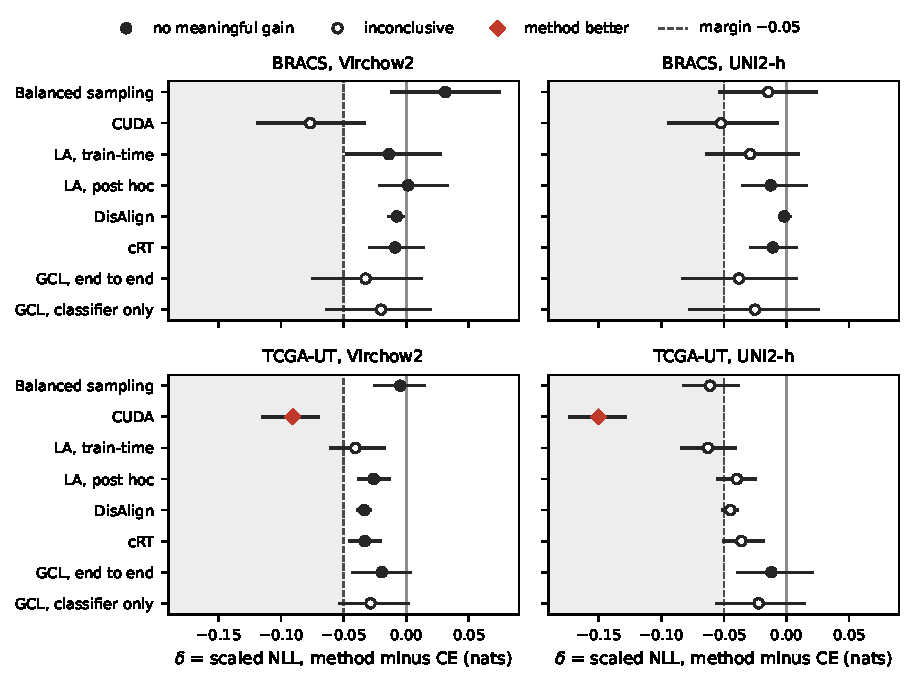
\includegraphics[width=\textwidth]{fig_contrasts.pdf}
\caption{Only CUDA on TCGA-UT improves on temperature-scaled CE by more than the margin. Paired difference $\delta$ in temperature-scaled NLL between each method and CE at $\rho=100$, with 99.84\% intervals (Bonferroni over 32 contrasts); negative values favour the method. The dashed line marks the margin $-0.05$ nats, the solid line zero, and the shaded band meaningful gains. CE: cross-entropy; LA: logit adjustment; CUDA: curriculum of data augmentation; DisAlign: distribution alignment; cRT: classifier re-training; GCL: Gaussian clouded logit adjustment.}
\label{fig:contrasts}
\end{figure}

\begin{table}[htbp]
\centering
\small
\renewcommand{\arraystretch}{1.15}
\begin{tabular}{@{}lrrrr@{}}
\toprule
 & BRACS & BRACS & TCGA-UT & TCGA-UT \\
Method & Virchow2 & UNI2-h & Virchow2 & UNI2-h \\
\midrule
\multicolumn{5}{@{}l}{\emph{Raw NLL minus scaled CE NLL (nats)}} \\
Balanced sampling & $2.19$ & $1.80$ & $0.36$ & $0.30$ \\
CUDA & $0.47$ & $0.46$ & $0.01$ & $-0.06$ \\
LA, train-time & $1.21$ & $1.20$ & $0.16$ & $0.17$ \\
LA, post hoc & $1.15$ & $1.09$ & $0.17$ & $0.17$ \\
DisAlign & $1.51$ & $1.86$ & $0.18$ & $0.22$ \\
cRT & $2.86$ & $2.24$ & $0.41$ & $0.35$ \\
GCL, end to end & $1.73$ & $2.11$ & $0.19$ & $0.55$ \\
GCL, classifier only & $1.93$ & $1.83$ & $0.10$ & $0.20$ \\
\midrule
\multicolumn{5}{@{}l}{\emph{Scaled ECE, method minus CE (points)}} \\
Balanced sampling & $-2.9$ & $-3.7$ & $-0.7$ & $-0.4$ \\
CUDA & $-2.9$ & $-3.4$ & $-1.0$ & $-1.6$ \\
LA, train-time & $-1.2$ & $-1.5$ & $-1.6$ & $-2.2$ \\
LA, post hoc & $0.0$ & $-0.9$ & $-1.7$ & $-2.6$ \\
DisAlign & $-0.5$ & $0.2$ & $-0.7$ & $-0.5$ \\
cRT & $-3.0$ & $-2.9$ & $-1.3$ & $-1.1$ \\
GCL, end to end & $-2.2$ & $-3.1$ & $-1.1$ & $-1.2$ \\
GCL, classifier only & $-2.3$ & $-3.6$ & $-1.9$ & $-1.8$ \\
\bottomrule
\end{tabular}
\caption{Without temperature scaling, no method except CUDA on TCGA-UT comes close to scaled CE; after scaling, almost every method is slightly better calibrated than CE. Point estimates at $\rho=100$ (descriptive). Top: raw NLL of each method minus scaled NLL of CE. Bottom: scaled expected calibration error (ECE) of each method minus that of CE. CE: cross-entropy; LA: logit adjustment; CUDA: curriculum of data augmentation; DisAlign: distribution alignment; cRT: classifier re-training; GCL: Gaussian clouded logit adjustment.}
\label{tab:secondary}
\end{table}
